\documentclass[twoside,11pt]{cergdoc}
\usepackage{graphicx}
\usepackage{amsmath}

\newcommand{\ITwoC}{I\textsuperscript{2}C }

\begin{document}

\title{XXBX Harness -- XBH}
\subtitle{XBH User Guide v1.0}
\author{Raghurama Velagala \and Matthew R. Carter \and Jens-Peter Kaps}
\email{jkaps@gmu.edu}
\affiliation{George Mason University\\
  Fairfax, Virginia}
\topicpic{xxbx-slide}

\maketitle

\tableofcontents

% -----------------------------------------------------------------------------
\chapter{Introduction}
% -----------------------------------------------------------------------------
At the same time, the EK-TM4C1294XL (Connected Launchpad) platform became available \cite{tm4c1294}.
This is a 120MHz board using the TM4C1294NCPDT (hereforth referred to as
TM4C1294), which is TI'S version of the 32-bit
ARM Cortex-M4F, with ethernet connectivity. There is 256kiB of SRAM and 1MiB of
ROM, which is far more than is available on the previous XBH. This board
typically runs software on bare metal (without an operating system), and is
suitable for realtime usage. It also has two built-in 12-bit ADCs capable of 2
million samples per second.

Ultimately the EK-TM4C1294XL was chosen due to the realtime capabilities and low
monetary cost, with the built-in ADC being a bonus.

% -----------------------------------------------------------------------------
\chapter{Measurements}
% -----------------------------------------------------------------------------
  \section{Timing}

A timing calibration service has been
implemented. When the XBS requests a 
timing calibration, the XBH triggers the
timing calibration routine on the XBD. This
routine busy loops for a device dependent
amount of time, toggles the timing outpout
digital I/O line as it does when 
benchmarking algorithms and additionally
counts the number of CPU cycles it spent
between the two digital I/O toggles using an
internal timer. This number of cycles is
reported to the XBH, which reports it along
with its owe timing measurement of the 
same event to the XBS. A 16-bit timer TC is
used to capture the timing flag from the XBD.
There might be a need for additional timer
TW at the same rate to get interrupts when timer
wraps around. Higher priority Timer Wraparound (TW)
counts wraps (w). TW can interrupt processing of
IT IST!. The Maximum time (t) is 35.8 seconds (64-bit
value) at 120\,MHz. Below you can see a timing
diagram for measuring timing properly.

\begin{figure}[ht]
  \begin{center}
    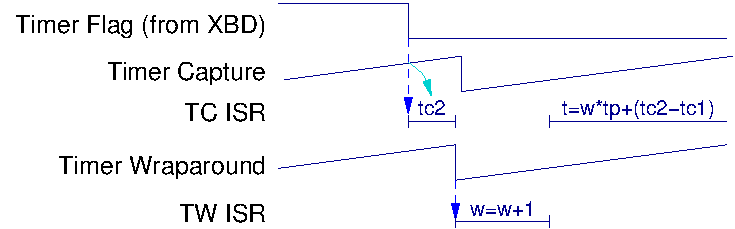
\includegraphics[scale=0.8]{figures/timing}
    \caption{Timing Measurements}\label{fig:timing}
  \end{center}
\end{figure}

Implementation for timing calibration (set GPIO low when running,
busy loop running for approximation 1\,sec,
exact number of cycles sent to the XBH), HAL
measures its timer to see how long it ran
during busy loop on XBD upload and hand
control over to target.

  \section{Power}



% -----------------------------------------------------------------------------
\chapter{Software}
% -----------------------------------------------------------------------------
  \section{Free RTOS}
The Tivaware package contains a version of FreeRTOS \cite{freertos}, which is an
RTOS licensed under the GNU Public License (GPL), with a linking exception for
proprietary drivers).  Alternative operating systems with support for the TM4C
and/or Cortex M4 are TI-RTOS and NuttX. FreeRTOS was chosen as it came with
the board support package with examples and was freely licensed, as well as
having support in the lwIP port for the TM4C1294.

The versions of both FreeRTOS and lwIP included in the Tivaware package was a
few versions behind. The version of FreeRTOS in Tivaware was 7.1, and the
version of lwIP was 1.4.1. We upgraded FreeRTOS to 8.2 and lwIP to the latest
from git. Upgrading lwIP required no changes besides copying the lwIP
port to the TM4C1294 provided by TI over, while upgrading FreeRTOS required
modifying the lwIP port provided by Tivaware. The benefit of updating to the
latest version is minimizing the delta of required changes in the future if a
feature is desired. The git version of lwIP provides dual-stack IPv6 and IPv4
which lwIP 1.4.1 does not support.

A problem we encountered was that the licensing for much of the Tivaware example
code was restrictive, prohibiting use with GPL'ed code and potentially causing
problems for redistribution \cite{tivaware-c}. Some of this example code was
needed to operate lwIP with FreeRTOS using the socket API, as it handled
initializing the ethernet hardware and GPIOs, notifying the lwIP stack of
incoming and transmitted ethernet frames, and setting up the IP address. This code had to be
replaced in order to not violate the license terms. We restricted our use of
Tivaware code to the driver library and the lwIP port which are freely licensed. 


    \subsection{Tasks}
The XBH software runs multiple tasks, which are managed by FreeRTOS and assigned
separate fixed-sized memory stacks. The tasks, in order of priority, from lowest to
highest, are
\begin{enumerate}
    \item lwIP TCP/IP
    \item XBH Server
\setcounter{enumi}{1}
    \item XBH command execution and XBD communication (same priority as XBH
        server)
    \item Ethernet Receive/Transmit - sends transmit and receive descriptors to
        lwIP.
    \item Power Measurement - woken up periodically by timer interrupt to
        perform measurements and enqueueing them to the XBH server task.
\end{enumerate}
Timeslicing is enabled, which makes FreeRTOS alternate between tasks of equal
priority without waiting for one to block. 

Execution time measurement is solely handled by interrupt handlers with the
timing values saved to global variables, and thus do not need a dedicated task.

The XBH Server task handles packets received from the XBS. It queues commands
onto the XBH command/XBD communication task for execution, and listens for
any reset command from the XBS while that thread executes. 

The XBH command/XBD communication task issues commands to the XBD and blocks
waiting for the XBD to complete the ordered operation and respond. 



The power measurement was separated into another task as we initially planned to
use the INA219 which used the \ITwoC bus, which does not immediately produce a result
when queried and thus is not suitable for direct querying by an interrupt
handler. The \ITwoC communication implementation polls the registers to determine if a
message has been sent, for reasons of simplicity, instead of having the task
sleep and woken up later by an interrupt indicating the \ITwoC task has been
completed. Using the FreeRTOS facilities is not an option, as it only has a
precision less than or equal to the tick period, which is 1ms  by default.

Instead, the power measurement task is woken by a timer interrupt on a
consistent interval, and as it is the highest priority task, will preempt other
FreeRTOS tasks. This task will do the polling of \ITwoC and enqueue the data to
the XBH server task for sending to the XBS.


This will not be necessary with the analog current shunt monitor, which can read the
value from the ADC register immediately and enqueue the value to be sent
directly into the XBH Server. 


    \subsection{Interrupts}
The TM4C1294 has 8 interrupt priority levels, 0-7. The meanings are inverted, with
priority 0 being the highest priority and priority 7 being the lowest, as with
other Cortex-M processors. The interrupt priorities are configured as follows,
from highest to lowest priority.
\begin{enumerate}
    \setcounter{enumi}{-1}
    \item Unused 
    \item Timer Wraparound
    \item Timer Capture 
    \item Max FreeRTOS SysCall Priority
    \setcounter{enumi}{2}
    \item Power Sample Timer
    \item Watchdog
    \item Unused 
    \item Unused 
    \item FreeRTOS kernel
\end{enumerate}

The timer wraparound interrupt is triggered when the 16-bit timer used for timer
capture wraps. The TM4C1294 uses is limited to 16-bit when used in edge-time
mode to capture the time that the start and stop signals are asserted. At
120MHz, a 16 bit timer is insufficient. Using equation \ref{eq:maxtime}, we get
546$\mu s$ before timer wrap which is shorter than the likely runtime.
\begin{equation}
    \label{eq:maxtime}
    \frac{1 }{f}\times 2^{n_{\rm bits}}
\end{equation}
$f$ is 120MHz, the clock rate we are running the board at, and $n_{\rm bits}$ is
the bits used to store the tick count, which is 16.

To work around this, a periodic timer that cycles at the same rate at higher priority is
used to count the number of times the edge timer has wrapped around \cite{tm4c1294}.
The interrupt handler for this will increment the count of wraps, or if it has
preempted the handler for the edge timer, will defer that incrementing for after
the completion of the edge timer interrupt, which records the computed time
since timer start into a 64-bit value. 64-bit is necessary, since by using equation
\ref{eq:maxtime} with 32 bits, we get a maximum time of 35.8 seconds, which is
also shorter than the potential longest time of execution.

The power sampling timer periodically issues an interrupt to record the current using a timer
synchronized to the wrap and capture timers as previously mentioned in
\ref{sec:xbh_tasks}.

The maximum syscall priority determines the minimum priority of the interrupts
that will be left enabled inside critical sections. Interrupt handlers that have
a priority higher than this cannot be preempted by FreeRTOS and cannot call
FreeRTOS API functions. 

The FreeRTOS kernel interrupts performs scheduling of FreeRTOS tasks and
initiates context switches when no other interrupts are pending and all
interrupts are unmasked. 


  \section{Lightweight IP}

lwIP (lightweight IP) is a widely
used open source TCP/IP stack designed
for embedded systems. The focus of the
lwIP TCP/IP implementation is to reduce
resource usage while still having a full-scale
TCP[1]. This makes lwIP suitable for use in
embedded systems with tens of kilobytes of
free RAM and room for around 40 kilobytes
of code ROM. The TivaWare [31] software
package intended for use with the EKTM4C1294XL
includes Lightweight IP
(lwIP) [32] and MicroIP (uIP), along with
drivers. 
 We decided to use lwIP as it
seemed to be under more active development, and came with the necessary drivers
for the TM4C1294.


  \section{XBS - XBH Protocol}
We only support TCP/IP, as opposed to TCP/IP and UDP/IP with the
        original XBH. There is no reason to support two different protocols, and
        TCP handles reliability and in-order delivery.

Messages are length prefixed. We are using TCP which is stream based
        and does not have a concept of messages, so we have to handle that
        ourselves. The previous XBX got away with not adding length prefixes
        because it assumed the application would only be notified of a message
        when the entire message was received, which is probably a fair
        assumption if the message is under the ethernet frame size and won't get
        fragmented. However, we opted to be strict and not allow for this
        assumption. Message payloads are also in binary format instead of text,
        to remove the need to decode hex on the XBH. 

  \section{Debug UART}


  \section{Toolchain}
We decided to use the GCC (GNU Compiler Collection) compiler as it was free and
easily available, and supported the ARM chip on the EK-TM4C1294XL. We decided to
use crosstool-ng in order to build GCC, along with newlib, which provides an
implementation of the standard C library.

% -----------------------------------------------------------------------------
\begin{appendix}
\chapter{XBS - XBH Protocol}


\end{appendix}

\end{document}
